\documentclass[12pt]{article}
 
\usepackage[margin=1in]{geometry} 
\usepackage{amsmath,amsthm,amssymb}
\usepackage{hyperref}
\usepackage{graphicx}
\usepackage{xcolor}
\usepackage[many]{tcolorbox}
\tcbuselibrary{listings}
\usepackage{listings}
\usepackage{subfig}

\usepackage{float}
\definecolor{lg}{HTML}{f0f0f0}

\newtcblisting{pycode}{
    colback=lg,
    boxrule=0pt,
    arc=0pt,
    outer arc=0pt,
    top=0pt,
    bottom=0pt,
    colframe=white,
    listing only,
    left=15.5pt,
    enhanced,
    listing options={
        basicstyle=\small\ttfamily,
        keywordstyle=\color{blue},
        language=Python,
        showstringspaces=false,
        tabsize=2,
        numbers=left,
        breaklines=true
    },
    overlay={
        \fill[gray!30]
        ([xshift=-3pt]frame.south west)
        rectangle
        ([xshift=11.5pt]frame.north west);
    }
}

\lstset{
    language=Python,
    basicstyle=\small\ttfamily,
}

 
\begin{document}
 
\title{Home Assignment 1}
\author{Cristian Manuel Abrante Dorta - 888248\\
CS-E4650 - Methods of data mining}

\maketitle
\section{Task 1}
\label{sec:task-1}

\subsection{Perform K-means and evaluate the goodness of clustering using
Silhouette Coefficient, Calinski Harabasz and Davies-Bouldin indices.
K = 2.}

An analysis of the results of the K-Means algorithm has been performed for three different values of K, and three indexes respectively. To reproduce the results, the random seed of the generator has been set to the value of $10$, obtaining the following results:

\begin{table}[h]
\centering
\begin{tabular}{c|ccc}
       & Avg. Silhouette coefficient & Calinski-Harabsz index & Davies-Bouldin score \\ \hline
$K = 2$  & 0.5587                 & 847.702                & 0.6216               \\
$K = 5$  & 0.4006                 & 778.4351               & 0.9299               \\
$K = 10$ & 0.3489                 & 593.5482               & 1.0729              \\

\end{tabular}
\caption{Results of different indexes for K = 2, K= 5 and K=10}
\label{tab:coefs}
\end{table}

\subsection{What is the optimal $K$ and why?}
\label{sec:optimal-k}

For answering this question, it is needed analysis of the performance of the K-means algorithm for each index, and each value of $K$.

\subsubsection{Silhouette coefficient}

The silhouette score indicates how each data point is close to the cluster it was matched by the algorithm, and how far it is from the other clusters (the neighbor clusters). This score varies from $[-1, +1]$, and can be calculated for each data point, as it is represented in Figures \ref{fig:sil-k-2}, \ref{fig:sil-k-5}, \ref{fig:sil-k-10}: \\

\begin{figure}[H]
   \begin{minipage}{0.32\textwidth}
     \centering
     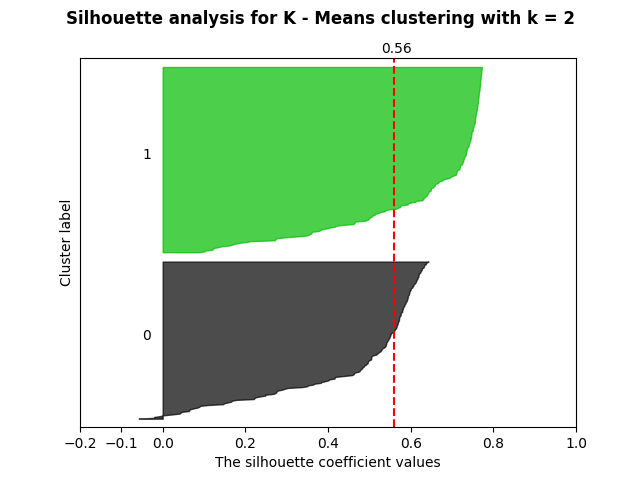
\includegraphics[width=\linewidth]{assignment-1/plots/task-1/silhouette-plot-k-2.png}
     \caption{$K = 2$}
     \label{fig:sil-k-2}
   \end{minipage}\hfill
   \begin{minipage}{0.32\textwidth}
     \centering
     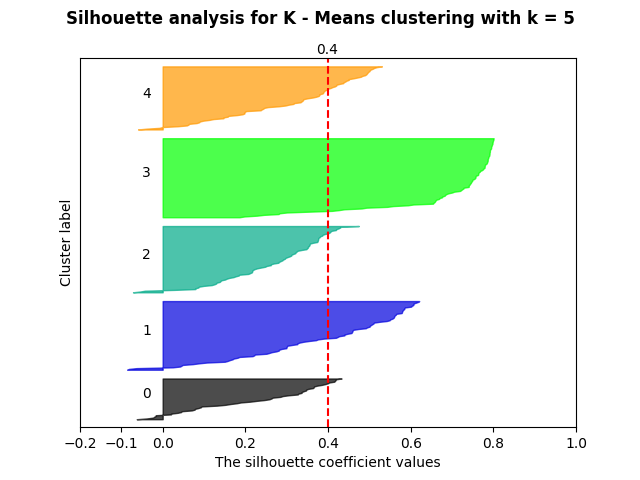
\includegraphics[width=\linewidth]{assignment-1/plots/task-1/silhouette-plot-k-5.png}
     \caption{$K = 5$}
     \label{fig:sil-k-5}
   \end{minipage}
   \begin{minipage}{0.32\textwidth}
     \centering
     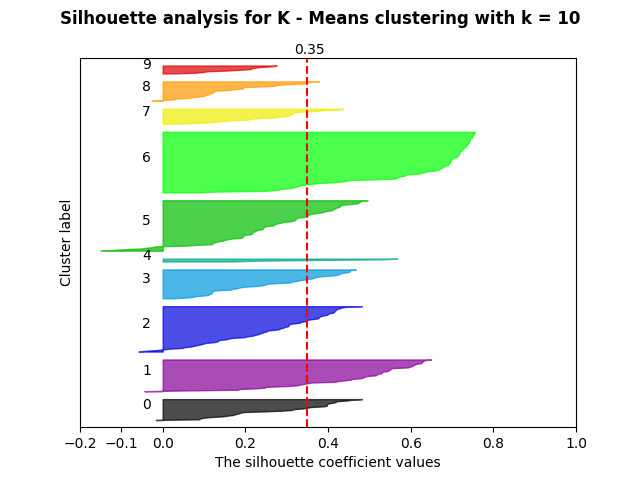
\includegraphics[width=\linewidth]{assignment-1/plots/task-1/silhouette-plot-k-10.png}
     \caption{$K=10$}
     \label{fig:sil-k-10}
   \end{minipage}
\end{figure}

Apart from the silhouette score for each data point, we can calculate the average for all the data points, which is the value shown in the first column of Table \ref{tab:coefs}. \\

The interpretation of the Silhouette score indicates that bigger values are better (close to $+1$), because when a big value is obtained it is an indication that the data points are closer to the cluster that they were assigned by the algorithm. The average score also follows this reasoning, having a better performance when it is higher.\\

If the averages values of the silhouette score are compared (Table \ref{tab:coefs}), it is shown that the value of $K=2$ is the better option with a value of $0.5587$, followed by $K=5$ with a value of $0.4006$ and finally $K=10$ with a value of $0.3489$. This can be also interpreted graphically, in the case of two clusters (Figure \ref{fig:sil-k-2}), we can see that most of the data points are well classified with values bigger than $0$ in almost all cases, except from some data points for cluster 0, which can be considered as outliers. For $K=5$ (Figure \ref{fig:sil-k-5}), there is also a good classification in most of the cases, but there are more points that have values smaller than $0$, on clusters 0,1,2 and 4. Finally, for $K=10$ (Figure \ref{fig:sil-k-10}), which is the worst result obtained in the average score, we can see that there are some points which are not well classified, especially in cluster 5, where some points have negatives values smaller than $-0.1$, also there are some clusters which are not well balanced in the proportion of points, and that is especially important in cluster 4, which do not contain almost data points.

\subsubsection{Calinski-Harabsz index}

This index is not measured for each data point as the silhouette score, but it is a unique value for all the datasets. The results obtained for different values of $K$ can be observed in the second column of Table \ref{tab:coefs}.\\

In the case of the Calinski-Harabsz index, as it indicates the ratio of dispersion between clusters and inter clusters, we can consider that bigger values are better. For our result, we can see that the best result is obtained for $K = 2$ with a value of 847.702, then followed by $K=5$ with a value of 778.4351 and finally $K=10$ with a value of 593.5482.

\subsubsection{Davis-Bouldin Index}

This index is more focused on measuring the separation between the specified clusters, this is why in this case lower values are better because they indicate less separation.\\

The results for this index could be seen in the third column of Table \ref{tab:coefs}. As in the previous indices, the best result is obtained by the execution with $K=2$ with a value of 0.6216, followed by the results of $K=5$ with a value of 0.9299, and finally, the worst performance is obtained by $K=10$ with a value of 1.0729.

\subsubsection{Selection of the optimal $K$}

According to the results obtained by all of the three indices, we can conclude that the best cluster performance is obtained for a value of $K=2$. It has the best performance for all three indices and also in the graphical representation of Figure \ref{fig:fig1}, we can see that almost all the data points are correctly clustered. \\

We can also add that, even though the value of $K=2$ is the one which offers the best performance, maybe for some domains are needed more clusters. In that case, we can say that $K=5$ offers the best trade-off between the number of clusters and evaluation performance.  

\section{Task 2}

\subsection{Perform hierarchical agglomerative clustering using different linkage metrics}

We have performed hierarchical clustering to the dataset using different linkage metrics. For each metric, a dendrogram was generated for showing how data is going to be grouped. Each dendogram is cut in the fourth level, for creating a clearer visualization. 

\begin{figure} [H]
\centering
\subfloat[Single-linkage metric]{
  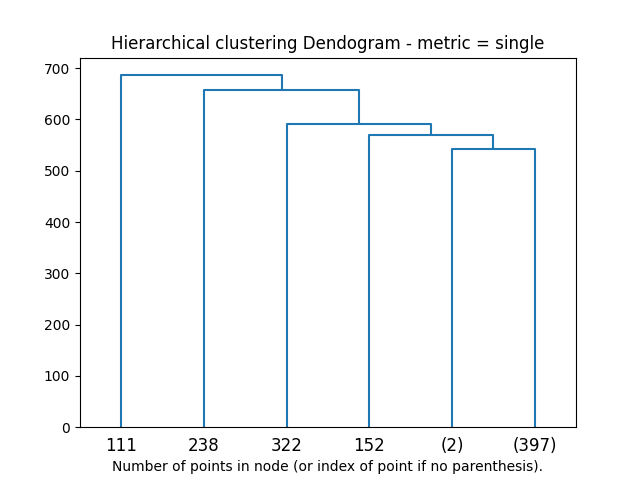
\includegraphics[width=65mm]{assignment-1/plots/task-2/dendogram-single-p4.png}
}
\subfloat[Complete-linkage metric]{
  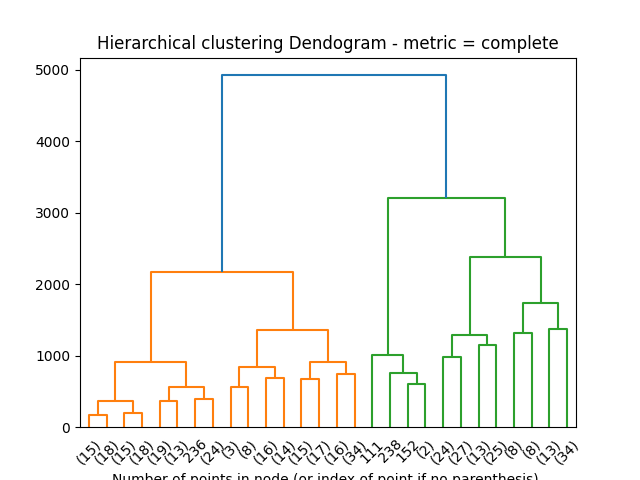
\includegraphics[width=65mm]{assignment-1/plots/task-2/dendogram-complete-p4.png}
}
\hspace{0mm}
\subfloat[Average-linkage metric]{
  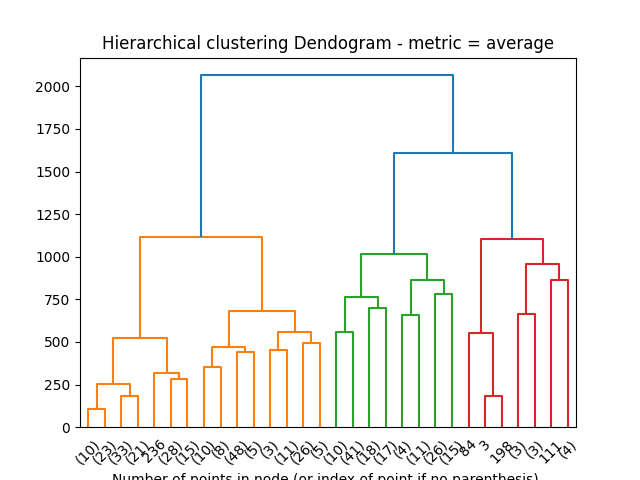
\includegraphics[width=65mm]{assignment-1/plots/task-2/dendogram-average-p4.png}
}
\subfloat[Distance of centroids metric]{
  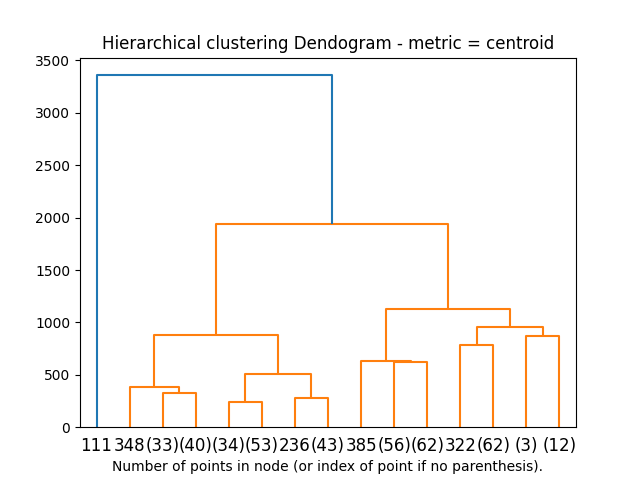
\includegraphics[width=65mm]{assignment-1/plots/task-2/dendogram-centroid-p4.png}
}
\hspace{0mm}
\caption{Dendograms of the resulting clustering for the four metrics}
\label{fig:hierarchical-clusters}
\end{figure}

\subsection{What is the optimal metric for this data and why?}

As in Section \ref{sec:optimal-k}, we have to select which is the algorithm (in this case which is the linkage metric), that performs best for our dataset. We have explored in previous sections three different indices for doing that: silhouette, Calinski-Haranasz, and Davies-Bouldin. To keep things simple, we are going to use in this case the Silhouette index for measuring the goodness of the clustering algorithm with different linkage metrics.

\begin{figure} [H]
\centering
\subfloat[Single-linkage metric]{
  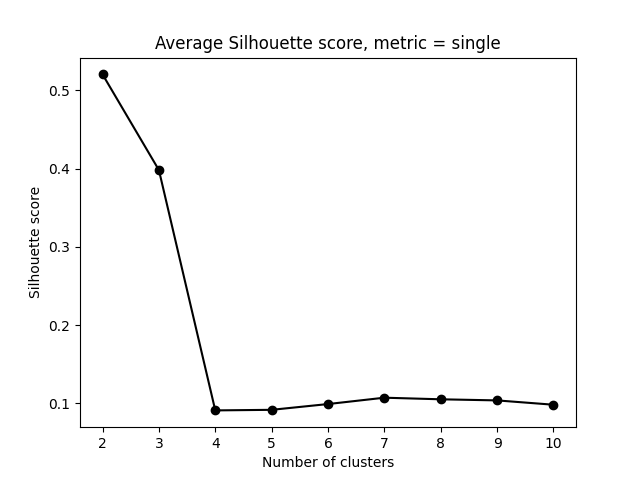
\includegraphics[width=65mm]{assignment-1/plots/task-2/silhouette-single.png}
}
\subfloat[Complete-linkage metric]{
  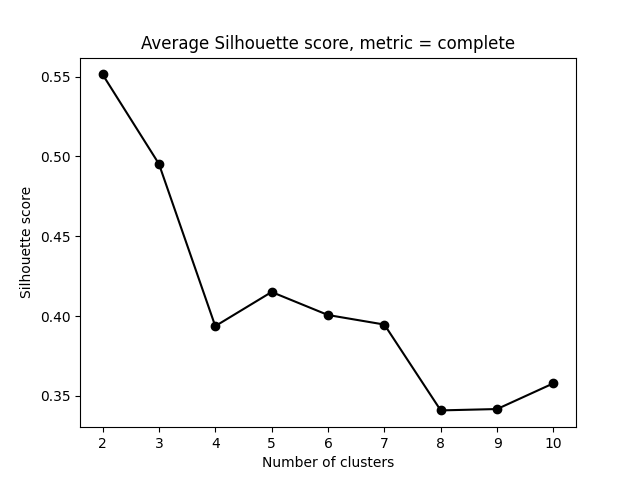
\includegraphics[width=65mm]{assignment-1/plots/task-2/silhouette-complete.png}
}
\hspace{0mm}
\subfloat[Average-linkage metric]{
  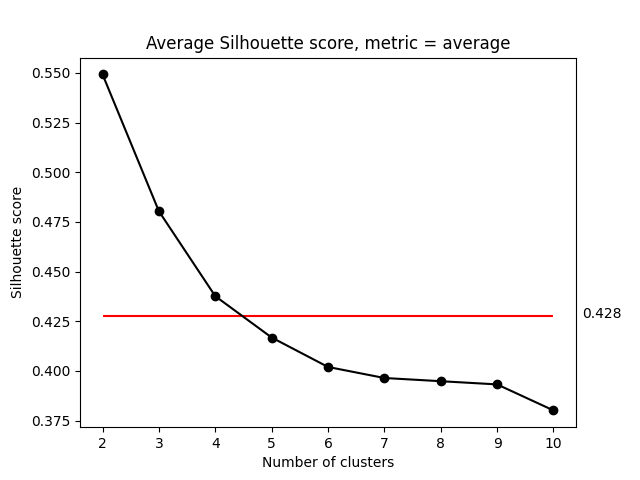
\includegraphics[width=65mm]{assignment-1/plots/task-2/silhouette-average.png}
}
\subfloat[Distance of centroids metric]{
  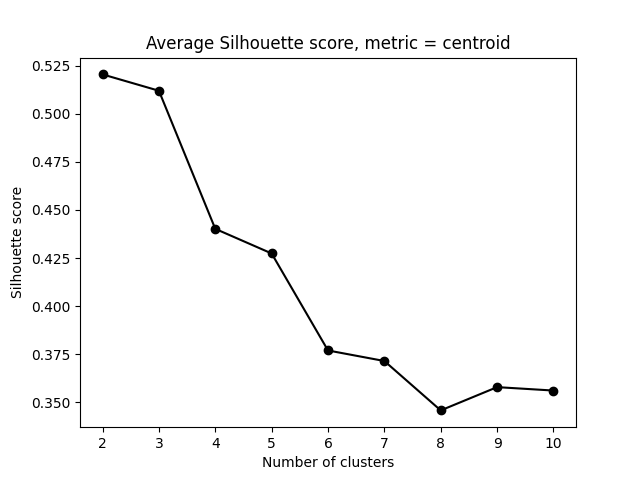
\includegraphics[width=65mm]{assignment-1/plots/task-2/silhouette-centroid.png}
}
\hspace{0mm}
\caption{Plot of the silhouette score for 1 to 10 clusters, for each of the metrics.}
\label{fig:sil-hierarchical}
\end{figure}

In figure \ref{fig:sil-hierarchical} we have created a plot of the performance of the hierarchical cluster algorithm according to silhouette score, with different linkage metrics. Additionally, we have plotted a horizontal line with the average value for all the clusters.\\

According to that, we can say that the metric that has the worst performance is the single metric, with an average score of 0.179, obtaining really bad results when the number of clusters is bigger than 3. With the other metrics, we obtain bigger values (around 0.4), obtaining the best of all them with the average linkage value of 0.428.\\ 

We can not say roundly that this is the best metric, because the other values are really close, but additionally, to have the best result in the metric, we can say that the plot is the most \textit{interpretable} of all of them, because the shape has fewer variations when the number of clusters varies.

\section{Task 3}

For experimenting, the dataset was shuffled five different times. Each time, the clustering algorithm was executed and the graphic representation in the form of a dendrogram was plotted. This was done for each linkage metric,in order to see the changes. In this case, we have plotted the dendrograms for the complete linkage metric (Figure \ref{fig:dendro-complete-linkage}):\\

\begin{figure}[H]
\centering
\subfloat[Shuffle 0]{
  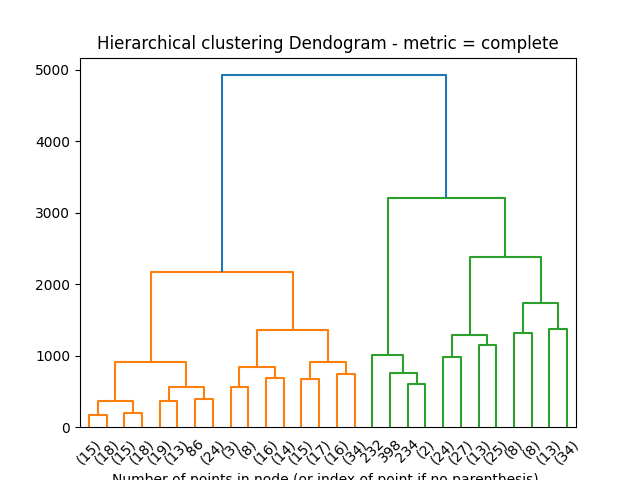
\includegraphics[width=65mm]{assignment-1/plots/task-3/dendogram-complete-0.png}
}
\subfloat[Shuffle 1]{
  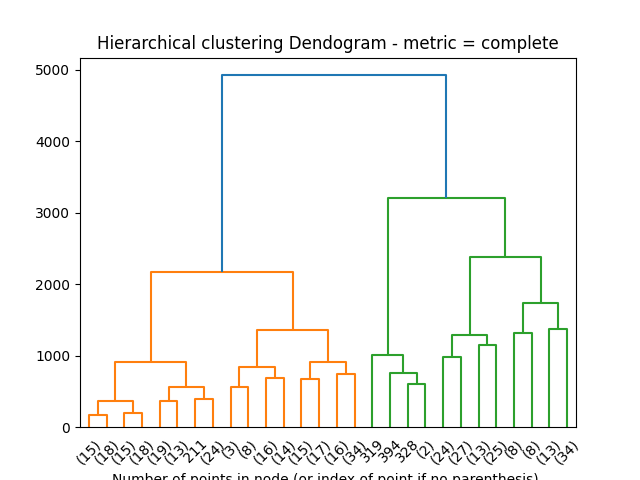
\includegraphics[width=65mm]{assignment-1/plots/task-3/dendogram-complete-1.png}
}
\hspace{0mm}
\subfloat[Shuffle 2]{
  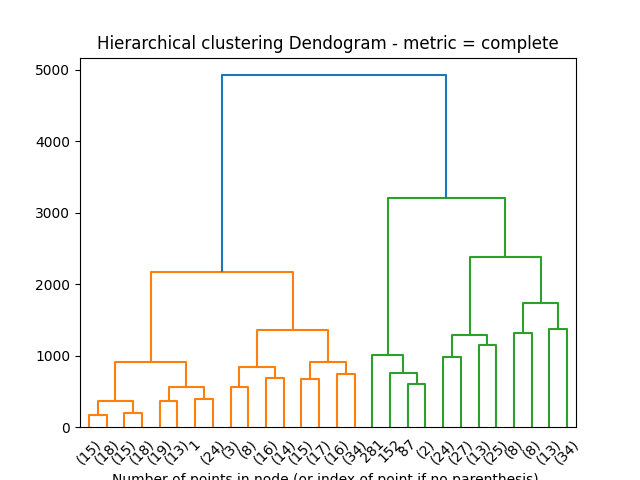
\includegraphics[width=65mm]{assignment-1/plots/task-3/dendogram-complete-3.png}
}
\subfloat[Shuffle 3]{
  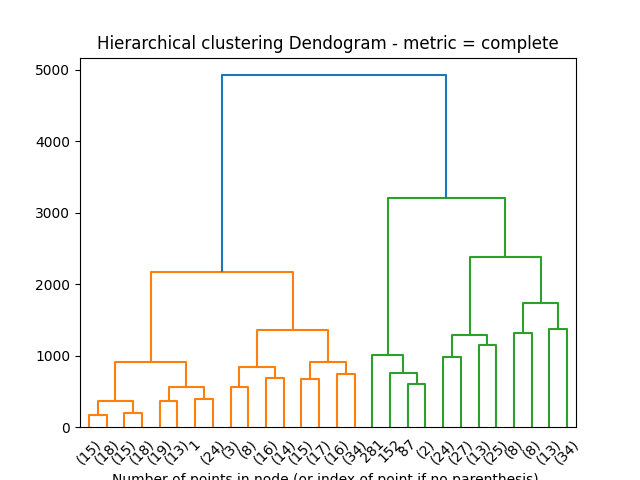
\includegraphics[width=65mm]{assignment-1/plots/task-3/dendogram-complete-3.png}
}
\hspace{0mm}
\subfloat[Shuffle 4]{
  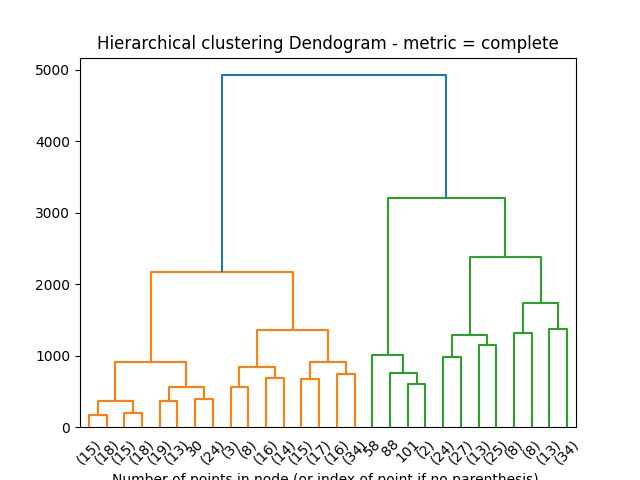
\includegraphics[width=65mm]{assignment-1/plots/task-3/dendogram-complete-4.png}
}
\caption{Dendrogram of different executions with complete linkage metric}
\label{fig:dendro-complete-linkage}
\end{figure}

We can see in the dendrogram representation that even that they hold the same structure, there are some changes in the leaf nodes (represented by numbers without parenthesis in the bottom). This is caused by the sensitivity of the metric to the order of the elements in the dataset.\\

When compared different metrics between each other we can see that there are metrics that are more robust to data order (like the complete linkage), and others that are sensitive to small changes, such as the single linkage metric, shown in Figure \ref{fig:dendro-single-linkage}:

\begin{figure}[H]
\centering
\subfloat[Shuffle 2]{
  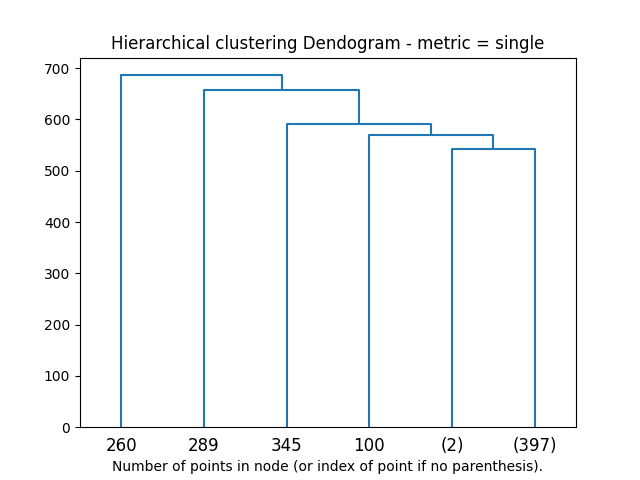
\includegraphics[width=65mm]{assignment-1/plots/task-3/dendogram-single-2.png}
}
\subfloat[Shuffle 4]{
  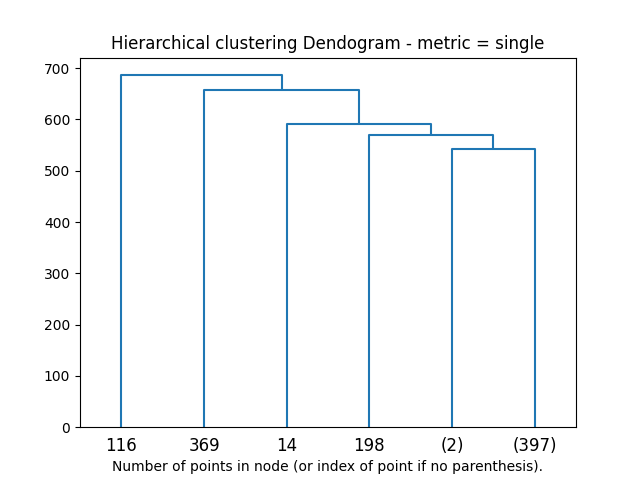
\includegraphics[width=65mm]{assignment-1/plots/task-3/dendogram-single-4.png}
}
\caption{Dendrogram of two different executions with single linkage metric}
\label{fig:dendro-single-linkage}
\end{figure}

Apart from observing the dendrograms, we can observe the different indices for measuring the quality of the cluster. In the experiment, the average value for all the metric does not change over the executions, which suggest that metrics does not vary depending on the position of the elements in the dataset.

\section{Task 4}

\subsection{Scale the numerical features as needed and calculate pairwise distances using only numerical features.}

The scale of numerical features have been performed using the min max-scale, so all the values have been reescaled to interval $[0-1]$.After that, the similarity graph was calculated, using euclidean distance (Figure \ref{fig:eucl-graph}):

\begin{figure}[h]
    \centering
    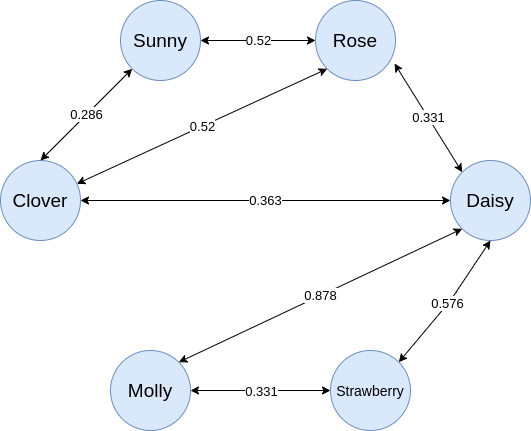
\includegraphics[scale=0.3]{assignment-1/plots/task-4/task-4-a-1.png}
    \caption{Similarity graph using euclidean distance.}
    \label{fig:eucl-graph}
\end{figure}

Also, it was calculated using the Mahalanobis distance (Figure \ref{fig:maha-graph}):

\begin{figure}[h]
    \centering
    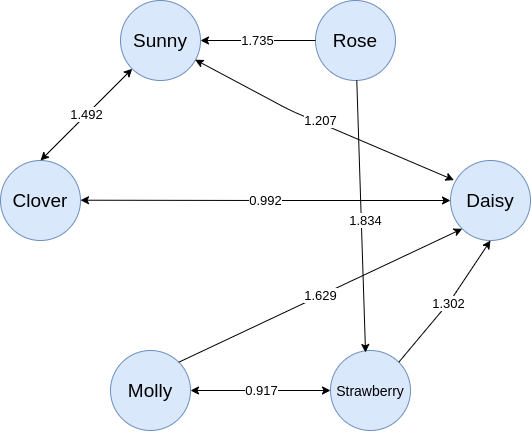
\includegraphics[scale=0.3]{assignment-1/plots/task-4/task-4-a-2.png}
    \caption{Similarity graph using Mahalanobis distance.}
    \label{fig:maha-graph}
\end{figure}

\subsection{Calculate pairwise similarities using only categorical features. Use
the Goodall measure.}

Using Goodall measure we have constructed the following similarity graph, connecting the two closest neighbors according to that measure (Figure \ref{fig:goodall-graph})

\begin{figure}[h]
    \centering
    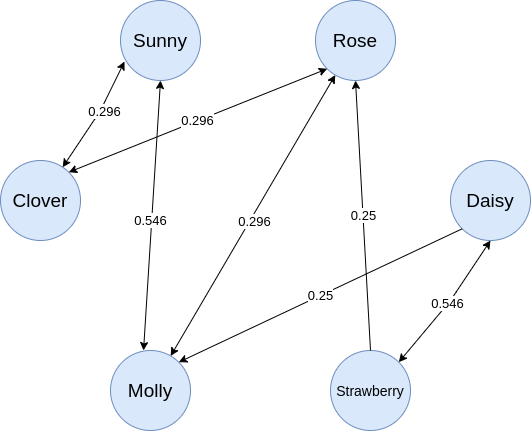
\includegraphics[scale=0.3]{assignment-1/plots/task-4/task-4-a-3.png}
    \caption{Similarity graph using Goodall measure.}
    \label{fig:goodall-graph}
\end{figure}

\subsection{Create a distance or similarity measure that combines the numerical and categorical measures so that neither group dominates.}

The similarity measure created, combines both the overlap similarity for categorical features and the euclidean distance for the numerical values. First of all, a preprocessing was made in the data in order to re-scale the numerical values (\textbf{age} and \textbf{milk/d}) into a $[0 - 1]$ scale. After that, categorical and numerical values were separated for performing the different calculations. The equation of the combined similarity was as it follows:

\begin{equation}
    s(x, y) = \lambda \cdot (\frac{1}{1 + L_2(x_{num}, y_{num}}) + (1-\lambda)\cdot(o(x_{cat}, y_{cat}))
    \label{eq:eq-meas}
\end{equation}

As we can see, the euclidean distance between numerical features ($L_2(x_{num}, y_{num})$), should be modified with a fraction. This is done for converting this distance measure into a similarity measure, and also for re-scaling the value into the same interval as the categorical features. \\

Using this measure of similarity, we calculated the similarity graph, representing the two nearest neighbors for each data point (Figure \ref{fig:combined-graph}):

\begin{figure}[h]
    \centering
    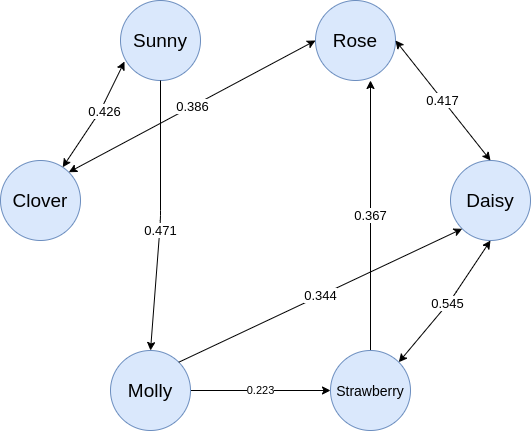
\includegraphics[scale=0.3]{assignment-1/plots/task-4/task-4-a-4.png}
    \caption{Similarity graph using combined measure.}
    \label{fig:combined-graph}
\end{figure}


\subsection{ If your combined measure was a similarity measure, present it as a distance measure.}

In equation \ref{eq:eq-meas} was presented the combined similarity measure for categorical and numerical data. With a small modification, it could be created also the measure for distance instead of similarity:

\begin{equation}
    d(x, y) = \lambda \cdot  L_2(x_{num}, y_{num}) + (1-\lambda)\cdot(1 - o(x_{cat}, y_{cat}))
    \label{eq:eq-dist}
\end{equation}

This small change in the overlap measure is correct because it is a scaled value in the interval $[0-1]$, so if all categorical features are the same, this value is going to be 1, so the distance is going to be zero. \\

For proving that this distance is a metric, we have to prove four different elements: \\

\textbf{$d(x, y) \ge 0$}\\

For proving that, we have to know that all elements in the distance are also going to be greater than zero. In the case of the euclidean distance, we know that this happens because all the measures of age and milk are greater than zero. The same happens with the overlapping measure, because in all the cases because it is defined that the minimum value is zero (with no elements in common). \\

\textbf{$d(x, y) = 0$ if and only if $x=y$}\\

In case that $x=y$ we can affirm that $L_2(x, y) = 0$, and $o(x, y) = 1$, so:

\begin{equation}
    d(x, y) = \lambda \cdot 0 + (1-\lambda) \cdot (1-1); 
d(x, y) = 0
\end{equation}

And that not could happen in other cases because if $x \neq y$ then or the euclidean distance is greater than zero (they are not in the same \textit{position}), or there is any categorical value that they do not share, so overlap measure is smaller than $1$. \\

\textbf{$d(x, y) = d(y, x)$}\\

We can prove that because we know that Euclidean distance is symmetrical and also overlapping measure, so the sum of both is going to be also symmetrical. \\

\textbf{$d(x, z) \leq d(y, x) + d(y, z)$}\\

We know that this property is held for the euclidean distance, but we have to prove it for this new metric. Making some abuse of the notation, we can write our expression as it follows:

\begin{equation}
    \lambda d_{xz} + (1-\lambda)(1-o_{xz}) \leq \lambda d_{xy} + (1-\lambda)(1-o_{xy}) + \lambda d_{yz} + (1-\lambda)(1-o_{yz}) 
\end{equation}

We know that the values of $d$ always hold the equation because it is the euclidean distance, but we have to take into account the case when the inequality could be broken. This case is when the $o_{xy}=1$ and $o_{yz}=1$, because that means that they are not going to add any extra value to the right part of the equation, so if $o_{xz} \neq 1$ then some value could be added to the left part, and the inequation could be broken. \\

But the characteristic of the overlapping measures does not allow that, because it is impossible that $o_{xy}=1$ and $0_{yz}=1$, it means that all the categorical values are the same between $x$ and $y$ and between $y$ and $z$, and then the categorical variables between $x$ and $z$ would be different, and thus the value will be different to 1. This happens because the number of variables is supposed to be the same for each data point.

\section{Task 5}

\subsection{ Carry out the principal component analysis of these data, that is, compute the eigenvalue decomposition of the corresponding sample covariance matrix.}

For computing the eigenvalues decomposition of the covariance matrix we have to follow some steps:

\begin{enumerate}
    \item \textbf{Standardize data}: \\
    Standarization means that the mean ($\mu=0$) and standard deviation ($\sigma=1$), for each feature column. For doing that we have followed the equation:
    \begin{equation}
        x_s^i = \frac{x^i - \mu_x^1}{\sigma_x}
    \end{equation}
    Before doing that we have to compute the average for column 1 ($\mu^1=\frac{1}{2}$) and for column 2 ($\mu^2=2$), and also the standard deviation for column 1 ($\sigma^1 = \sqrt{\frac{5}{8}}$) and for column 2 ($\sigma^1 = \sqrt{\frac{5}{8}}$). The standardized matrix then is:
    \begin{equation}
    X =
        \begin{pmatrix}
         -\frac{\sqrt{10}}{5} & -\frac{2\sqrt{10}}{5} \\
         -\frac{2\sqrt{10}}{5} & -\frac{\sqrt{10}}{5} \\
         \frac{2\sqrt{10}}{5} & \frac{\sqrt{10}}{5} \\
         \frac{\sqrt{10}}{5} & \frac{2\sqrt{10}}{5} \\
        \end{pmatrix}
    \end{equation}
    
    \item \textbf{Calculate covariance matrix}\\
    As we have previously standardized the values, we can compute the covariance matrix, in a simple way, following this formula:
    \begin{equation}
        cov = \frac{1}{n-1}X^TX
    \end{equation}
    This gives us the following covariance matrix as result:
    \begin{equation}
    cov =
        \begin{pmatrix}
         \frac{4}{3} & \frac{16}{15} \\
          \frac{16}{15} &\frac{4}{3} \\
        \end{pmatrix}
    \end{equation}
    \item \textbf{Compute eigenvalues}      
    For computing the eigenvalues of the matrix, we have to compute the following matrix first:
    \begin{equation}
        X - \lambda I
    \end{equation}
    Where, $\lambda$ is going to be the eigenvalues of the matrix. In our case:
    \begin{equation}
        X - \lambda I =
        \begin{pmatrix}
         \frac{4}{3} - \lambda & \frac{16}{15} \\
          \frac{16}{15} &\frac{4}{3} - \lambda \\
        \end{pmatrix}
    \end{equation}
    After that, we should compute the determinant of the matrix:
    \begin{equation}
        det(X - \lambda I) = det\begin{pmatrix}
         \frac{4}{3} - \lambda & \frac{16}{15} \\
          \frac{16}{15} &\frac{4}{3} - \lambda \\
        \end{pmatrix} = (\frac{4}{13}-\lambda)^2-(\frac{16}{15})^2
        =\lambda^2-\frac{8}{3}\lambda+\frac{16}{25}
    \end{equation}
    We then calculate the values of $\lambda$ that solve the equation, and those values are going to be the eigenvalues of the matrix.
    \begin{equation}
        \lambda^2-\frac{8}{3}\lambda+\frac{16}{25}=0
    \end{equation}
    The solutions are $\lambda_1 = \frac{12}{5}=2.4$ and $\lambda_2=\frac{4}{15}=0.2666$
    
    \item \textbf{Compute the corresponding eigenvectors}:\\
    
    We compute the corresponding eigenvectors for each eigenvalue:
    \begin{itemize}
        \item \textbf{$\lambda_1=\frac{12}{5}$}:\\
        The corresponding eigenvector should satisfy:
        \begin{equation}
            \begin{pmatrix}
             \frac{4}{3} & \frac{16}{15} \\
              \frac{16}{15} &\frac{4}{3} \\
            \end{pmatrix}
            \begin{pmatrix}
                x_1 \\ x_2
            \end{pmatrix} = \frac{12}{5}
            \begin{pmatrix}
                x_1 \\ x_2
            \end{pmatrix}
        \end{equation}
        If n the equation mode, the value that we should solve is:
        \begin{equation}
            \begin{split}
                \frac{8}{15}x_1+\frac{16}{15}x_2=0 \\
                \frac{16}{15}x_1+\frac{8}{15}x_2=0
            \end{split}
        \end{equation}
        Which gives as a result the solution of $x_1=x_2$, which we can consider $k$, for simplifying. It is desirable to have a normalized value, so it has to satisfy:
        \begin{equation}
            k^2+k^2=1
        \end{equation}
        So then the value of $k=\frac{\sqrt{2}}{2}$, and the corresponding eigenvector $v_1=\begin{pmatrix}\frac{\sqrt{2}}{2} \\ \frac{\sqrt{2}}{2}\end{pmatrix}$
        \item \textbf{$\lambda_2=\frac{4}{15}$}:\\
        The corresponding eigenvector should satisfy:
        \begin{equation}
            \begin{pmatrix}
             \frac{4}{3} & \frac{16}{15} \\
              \frac{16}{15} &\frac{4}{3} \\
            \end{pmatrix}
            \begin{pmatrix}
                x_1 \\ x_2
            \end{pmatrix} = \frac{4}{15}
            \begin{pmatrix}
                x_1 \\ x_2
            \end{pmatrix}
        \end{equation}
        If n the equation mode, the value that we should solve is:
        \begin{equation}
            \begin{split}
                \frac{16}{15}x_1+\frac{16}{15}x_2=0 \\
                \frac{16}{15}x_1+\frac{16}{15}x_2=0
            \end{split}
        \end{equation}
        Which gives as a result the solution of $x_1=-x_2$, which we can consider $k$, for simplifying. It is desirable to have a normalized value, so it has to satisfy:
        \begin{equation}
            k^2+k^2=1
        \end{equation}
        So then the value of $k=\frac{\sqrt{2}}{2}$, and the corresponding eigenvector $v_1=\begin{pmatrix}-\frac{\sqrt{2}}{2} \\ \frac{\sqrt{2}}{2}\end{pmatrix}$
    \end{itemize}
    
    
\end{enumerate}

\subsection{Consider the resulting decomposition:}

\subsubsection{Use it to transform the original 2-dimensional data set into a 1-dimensional representation (a 4 × 1 matrix) such that the variance of the resulting data is equal to the largest eigenvalue.}

We can use the eigenvector corresponding to the bigger eigenvalue ($\lambda_1=\frac{12}{5}$), to transform the original standardized data in order to preserve the maximum amount of variance possible:

\begin{equation}
    X \begin{pmatrix} \frac{\sqrt{2}}{2} \\ \frac{\sqrt{2}}{2}\end{pmatrix} = 
    \begin{pmatrix}
        -\frac{3\sqrt{5}}{5} \\
        -\frac{3\sqrt{5}}{5} \\
        \frac{3\sqrt{5}}{5} \\
        \frac{3\sqrt{5}}{5}
    \end{pmatrix}
\end{equation}

If we calculate the variance we can see that $\sigma=\frac{12}{5}$, corresponding to the biggest eigenvalue.

\subsubsection{Next, use it to transform the original data set into a 2-dimensional representation, such that the variance of one of the columns is equal to the smallest eigenvalue.}

For doing this transformation ,we multiply the original data with the two obtained eigenvectors, obtaining as a result a 4x1 matrix, where the second column has as variance the value of the smallest eigenvalue:

\begin{equation}
    X 
    \begin{pmatrix} 
        \frac{\sqrt{2}}{2} & -\frac{\sqrt{2}}{2} \\ 
        \frac{\sqrt{2}}{2} & \frac{\sqrt{2}}{2}
    \end{pmatrix} 
    = 
    \begin{pmatrix}
        -\frac{3\sqrt{5}}{5} & -\frac{\sqrt{5}}{5} \\
        -\frac{3\sqrt{5}}{5} & \frac{\sqrt{5}}{5}  \\
        \frac{3\sqrt{5}}{5}  & -\frac{\sqrt{5}}{5} \\
        \frac{3\sqrt{5}}{5}  & \frac{\sqrt{5}}{5}
    \end{pmatrix}
\end{equation}

\subsection{Given two points in $d$-dimensional Euclidean space}:

\subsubsection{Compute the Euclidean distance between all pairs of points in the original data set.}

We can represent those distances in a matrix where each row and column are a certain point, and the positions ($i$, $j$) is the distance between $p_i$ and $p_j$:

\begin{equation}
    \begin{matrix}
        0.0 & 0.8944 & 2.6832 & 2.8284 \\
        0.8944 & 0.0 & 2.8284 & 2.6832 \\
        2.6832 & 2.8284 &  0.0 & 0.8944 \\
        2.8284 & 2.6832 &  0.8944 & 0.0    
    \end{matrix}
\end{equation}

As we can see this is a simetric matrix, because Euclidean distance is a metric.

\subsubsection{Compute the Euclidean distance between all pairs of points in the 1-dimensional representation obtained in exercise 5b.}

\begin{equation}
    \begin{matrix}
        0.0 & 0.0 & 2.6832 & 2.6832 \\
        0.0 & 0.0 & 2.6832 & 2.6832 \\
        2.6832 & 2.6832 &  0.0 & 0.0 \\
        2.6832 & 2.6832 &  0.0 & 0.0    
    \end{matrix}
\end{equation}

\subsubsection{Compute the Euclidean distance between all pairs of points in the 2-dimensional representation obtained in exercise 5b.}

\begin{equation}
    \begin{matrix}
        0.0 & 0.8944 & 2.6832 & 2.8284 \\
        0.8944 & 0.0 & 2.8284 & 2.6832 \\
        2.6832 & 2.8284 &  0.0 & 0.8944 \\
        2.8284 & 2.6832 &  0.8944 & 0.0    
    \end{matrix}
\end{equation}

\subsubsection{What is the effect of the previous transformations on these distances?}

We can see that the distance between data points does not differ between the original data and the second transformation. That makes sense, because we are not modifying the distances between the data points, but only changing the axis to where they refer to. \\

Also we can see that in the second transformation some distances are lost, and that is also reasonable because as we are making a projection over the eigenvector, so we are losing some information. 

\subsection{Repeat exercises 5a and 5b on these data.}

We are going to copy the same steps as in the previous sections:
\begin{enumerate}
    \item \textbf{Standardize data}: \\
    Standarized data is:
    
    \begin{equation}
    X =
        \begin{pmatrix}
         -1 & -1 \\
         -1 & 1 \\
         1 & -1 \\
         1 & 1 \\
        \end{pmatrix}
    \end{equation}
    
    \item \textbf{Calculate covariance matrix}\\
   
    This gives us the following covariance matrix as result:
    \begin{equation}
    cov =
        \begin{pmatrix}
         1.33 & 0.0 \\
         0.0 & 1.33 \\
        \end{pmatrix}
    \end{equation}
    \item \textbf{Compute eigenvalues}      
    For computing the eigenvalues of the matrix, we have to compute the following matrix first:
    \begin{equation}
        X - \lambda I
    \end{equation}
    Where, $\lambda$ is going to be the eigenvalues of the matrix. In our case:
    \begin{equation}
        X - \lambda I =
        \begin{pmatrix}
         1.33 - \lambda & 0 \\
          0 &1.33 - \lambda \\
        \end{pmatrix}
    \end{equation}
    After that, we should compute the determinant of the matrix:
    \begin{equation}
        det(X - \lambda I) = det\begin{pmatrix}
         1.33 - \lambda & 0 \\
          0 &1.33 - \lambda \\
        \end{pmatrix}
    \end{equation}

    The solutions are $\lambda_1 = 1.33$ and $\lambda_2=1.33$
    
    \item \textbf{Compute the corresponding eigenvectors}:\\
    
    We compute the corresponding eigenvectors for each eigenvalue:
    \begin{itemize}
        \item \textbf{$\lambda_1=1.33$}:\\
        
        The corresponding eigenvector $v_1=\begin{pmatrix}1 \\ 0\end{pmatrix}$
        \item \textbf{$\lambda_1=1.33$}:\\
        
        The corresponding eigenvector $v_1=\begin{pmatrix}0 \\ 1\end{pmatrix}$
    \end{itemize}
    
    
\end{enumerate}


\end{document}
